\section{Security Layer}

\subsection{AES-256-GCM Encrypted Storage}

The \texttt{SecureKeyStorage} module provides encrypted storage for private key material using AES-256-GCM~\cite{nist2007aesgcm}. All sensitive data (Ed25519 private keys, X25519 private keys, channel session keys) is encrypted before storage and decrypted on demand, ensuring that even if the in-memory store is compromised, the attacker obtains only ciphertext.

The encryption pipeline: (1) Generate a random 96-bit nonce per encryption operation; (2) Encrypt the plaintext with AES-256-GCM using the master key; (3) Store the ciphertext + nonce + authentication tag; (4) Decrypt on demand using the same master key and nonce. The GCM mode provides both confidentiality and integrity: any tampering with the ciphertext or nonce causes decryption to fail with an authentication error.

AES-256-GCM latency scales linearly with data size: 1.01\textmu s for 16 bytes, 1.98\textmu s for 256 bytes, 5.11\textmu s for 1KB, 16.40\textmu s for 4KB, and 61.99\textmu s for 16KB. The linear scaling ($\approx$ 3.7\textmu s per KB) indicates that the encryption overhead is dominated by the block processing cost rather than the nonce/tag overhead, making AES-GCM practical for all key storage sizes in Nexa-net (Ed25519 keys are 32 bytes, encrypted in $\approx$1.3\textmu s).

\subsection{DashMap-Based Lock-Free Rate Limiting}

The \texttt{RateLimiter} module implements per-DID rate limiting using DashMap~\cite{dashmap2022}, a lock-free concurrent hash map. The rate limiter tracks request counts per DID within fixed time windows (e.g., 1000 requests per minute per DID). Each rate limit check performs: (1) Look up the DID's entry in the DashMap (lock-free read); (2) Check if the current count exceeds the limit; (3) Atomically increment the count if under the limit, or reject the request if over.

The migration from \texttt{RwLock<HashMap>} to DashMap eliminated read-lock starvation under high concurrency. In the previous implementation, concurrent rate limit checks required acquiring a read lock, which blocked when a writer (count increment) held the write lock. DashMap's sharded internal design (each shard is an independent \texttt{RwLock}) ensures that concurrent reads on different DIDs never contend, and writes affect only the relevant shard.

Rate limit checks benchmark at approximately 1\textmu s per check, negligible compared to the 30\textmu s semantic routing latency. The DashMap approach supports the expected concurrency level (1000+ simultaneous agents) without performance degradation.

\subsection{AuditLogger}

The \texttt{AuditLogger} records all security-relevant events in a tamper-evident log. Each log entry includes: timestamp, event type (authentication, channel operation, receipt signing, rate limit violation), actor DID, target DID, operation details, and outcome (success/failure with error code).

The audit log is append-only: entries can be added but never modified or deleted. Log integrity is verified through a running SHA-256 hash chain (similar to the receipt hash chain), where each entry's hash incorporates the previous entry's hash. This makes any tampering detectable by recomputing the chain and comparing against the stored hashes.

Audit throughput benchmarks at variable rates depending on log storage backend. The default implementation uses in-memory \texttt{Vec<AuditEntry>} with periodic hash chain verification, suitable for development and testing. Production deployment would use a persistent append-only store (e.g., RocksDB~\cite{rocksdb2014} or PostgreSQL) with the same hash chain integrity guarantee.

\subsection{KeyRotator}

The \texttt{KeyRotator} manages periodic rotation of cryptographic keys. Key rotation follows a three-phase process:

\begin{enumerate}
  \item \textbf{Announcement}: Publish a new DID Document with the new verification method, keeping the old method marked as \texttt{revoked: pending}. This allows existing sessions to continue using the old key while new sessions adopt the new key.
  \item \textbf{Transition}: After a grace period (configurable, default 24 hours), stop accepting new authentication attempts with the old key. Existing channels can continue until they close naturally.
  \item \textbf{Finalization}: Remove the old key from the DID Document. All sessions using the old key are terminated, and the old private key material is zeroized~\cite{zeroize2022}.
\end{enumerate}

The key rotation design ensures zero downtime: the overlap period between announcement and finalization allows all active sessions to complete their lifecycle before the old key is revoked. The rotation schedule is configurable per key type: signing keys rotate every 90 days, key agreement keys rotate every 30 days, and the master identity key rotates only on manual trigger (requiring DID Document re-publishing).

\subsection{SecurityManager Coordinator}

The \texttt{SecurityManager} acts as the coordinator for all security subsystems. It provides a unified interface for security operations: \texttt{verify\_identity(did)}, \texttt{check\_rate\_limit(did)}, \texttt{log\_audit(event)}, and \texttt{rotate\_key(key\_type)}. The SecurityManager orchestrates the interactions between SecureKeyStorage, RateLimiter, AuditLogger, and KeyRotator, ensuring that security checks are applied consistently across all four protocol layers.

For example, when a new RPC session is established, the SecurityManager: (1) verifies both parties' DIDs via the DID resolver; (2) checks rate limits for both DIDs; (3) logs the session establishment event; and (4) provides the session's encryption keys from SecureKeyStorage. This coordination ensures that no session bypasses any security check---a single missed step would be a security vulnerability.

\begin{figure}[t]
\centering
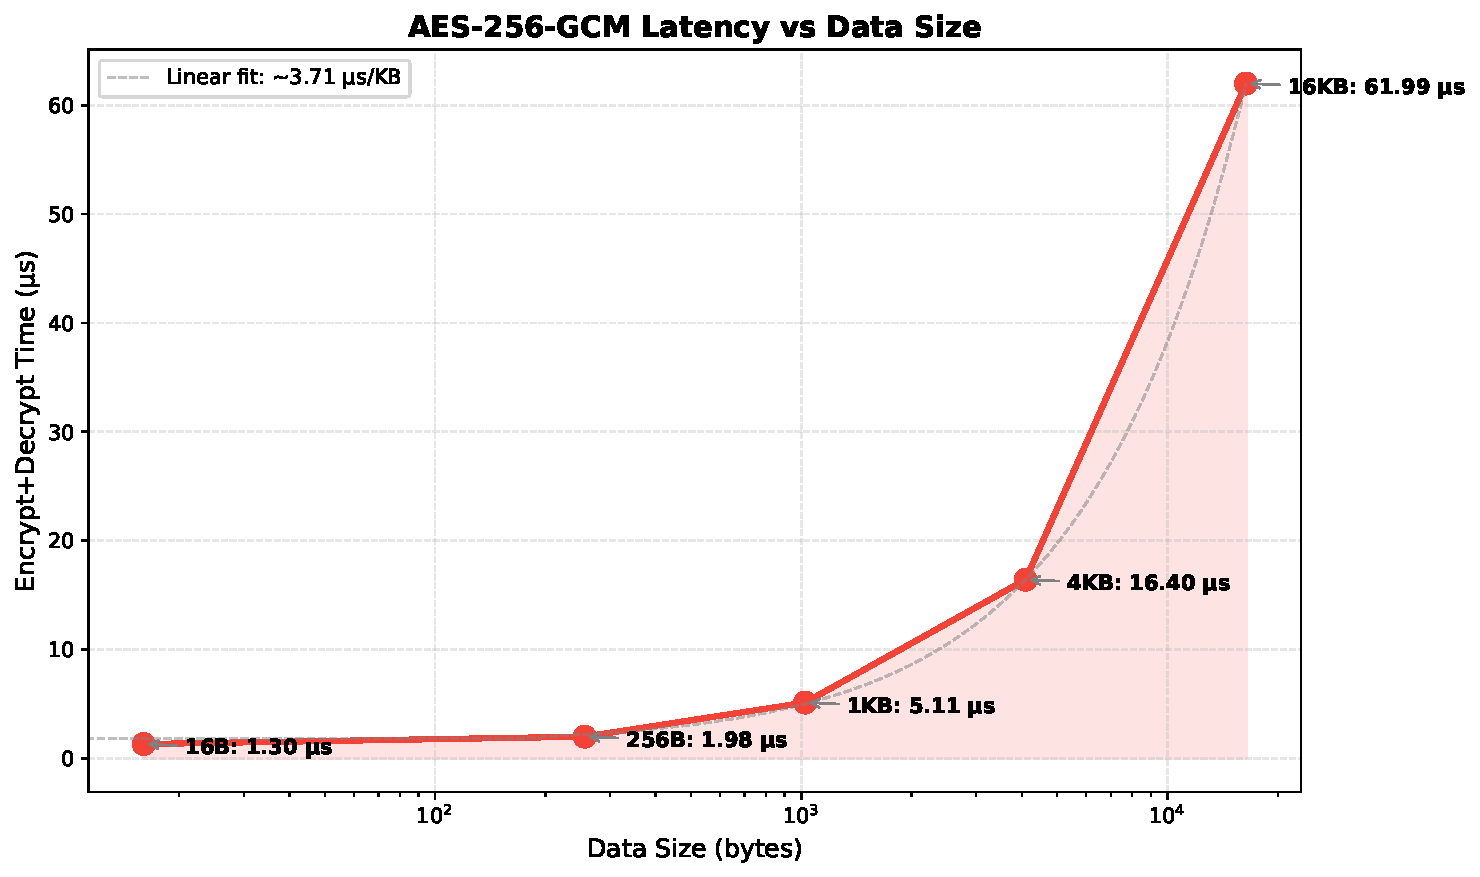
\includegraphics[width=0.85\columnwidth]{figures/security_bench.pdf}
\caption{AES-256-GCM latency vs data size. Linear scaling at $\approx$3.7\textmu s/KB makes encryption practical for all key sizes.}
\label{fig:security-bench}
\end{figure}